\chapter{Grundlagen} % 15 Seiten

Die Vermittlung der Grundlagen dient als Basis für die weitere Arbeit und beginnt mit einer Erläuterung der verschiedenen Vorgehensmodelle.
Darauf folgt eine Einführung in DevOps bevor das Kapitel mit einem Vergleich der klassischen und sicherheitskritischen Bereiche abschließt.

\section{Vorgehensmodelle} % 6 Seiten

Diese Arbeit kategorisiert die Vorgehensmodelle zur Entwicklung von Software in zwei Kategorien: \emph{klassische} und \emph{agile} Vorgehensmodelle.
Unter \emph{klassisch} werden alle Vorgehensmodelle, die nicht agil und somit (vornehmlich) plangetrieben sind, zusammengefasst.
Im Fokus dieses Abschnitts steht die Erläuterung relevanter Vertreter dieser Kategorien.

\subsection{Klassisch} % 3 Seiten

Nachfolgend sollen einige wichtige klassische iterative als auch nicht-iterative Vorgehensmodelle kurz vorgestellt werden.

\subsubsection{Wasserfallmodell}

Das Wasserfallmodell wird konzeptionell das erste mal in \parencite[][]{Royce:1970aa} beschrieben.
Es beschreibt ein rein sequentielles Vorgehen in der Entwicklung (vgl. \autoref{fig:wasserfallmodell}). 
Dabei fließt der Output einer vorgelagerten Stufe stets als Input in die nachgelagerte Stufe.

\begin{figure}
  \centering
  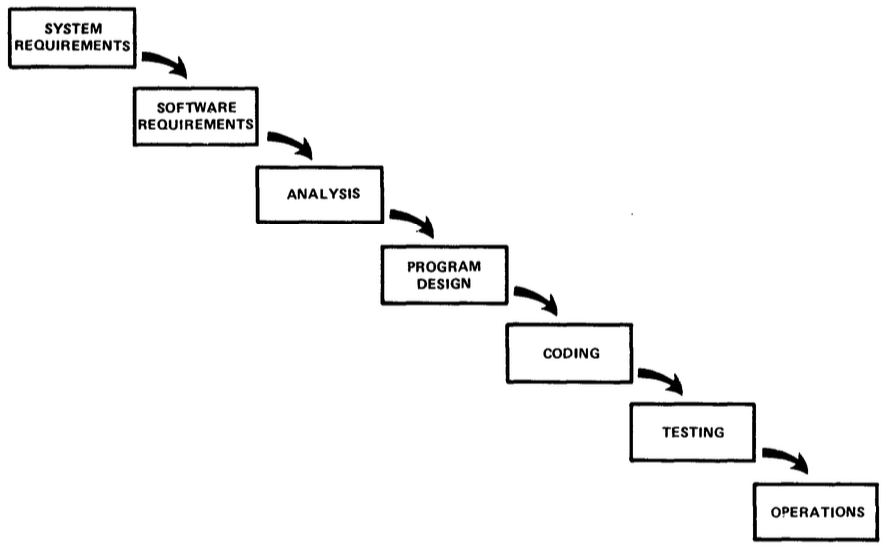
\includegraphics[width=\textwidth]{img/wasserfallmodell.png}
  \caption{Grundlegendes Wasserfallmodell \parencite[][]{Royce:1970aa}}
  \label{fig:wasserfallmodell}
\end{figure}

Dieses Modell weist eine sehr gute Planbarkeit auf, da es streng abgegrenzte Phasen gibt. 
Bezeichnend ist, dass die jeweiligen Phasen stets vollständig abgeschlossen sein müssen, bevor zu der nächsten Phase übergegangen wird \parencite[vgl.][S. 48]{Schatten:2010aa}.
Erweiterungen des Modells bestehen in der Einführung einer Rücksprungmöglichkeit, wenn in einer Phase Fehler erkannt oder sonstige Richtlinien verletzt werden.
Dieses sequentielle Vorgehen hat den Nachteil, dass der Kunde lediglich am Anfang und am Ende in den Entwicklungsprozess miteinbezogen wird, sowie Änderungswünsche während der Entwicklung nicht berücksichtigt werden können.
Auch das Auftreten von Risiken verzögert den Projektverlauf, da alle nachgelagerten Phasen betroffen sind.

Dass dieses Modell für große Softwareprojekte meist wenig geeignet ist, wurde bereits 1970 erkannt: \enquote{In my experience, however, the simpler method has never worked on large software development efforts [...]} \parencite[][S. 335]{Royce:1970aa}.

Mittlerweile wird dieses Vorgehen für moderne Softwareprojekte kaum noch verwendet und aktuelle Literatur rät auch meist von der Verwendung des Modells ab.
\parencite[Vgl.][S. 49]{Schatten:2010aa}

\subsubsection{Spiralmodell}

Das Spiralmodell ist ein iterative-inkrementelles, risikogetriebenes Vorgehensmodell.
Dabei werden die Entwicklungsschritte zyklisch durchlaufen (vgl. \autoref{fig:spiralmodell}), bis das Endprodukt fertiggestellt ist.
Entstanden ist das Modell aus dem Wasserfallmodell, welches angepasst für umfangreiche Regierungsprojekte verwendet wurde \parencite[vgl.][S. 64]{Boehm:1988aa}.
\parencite[][S. 57]{Schatten:2010aa} identifiziert dabei die folgenden vier Schritte als Hauptbestandteile des Spiralmodells:

\begin{itemize}
\item Zieldefinition
\item Risikoeinschätzung
\item Testen
\item Feedback und Planung der nächsten Iteration
\end{itemize}

\begin{figure}
  \centering
  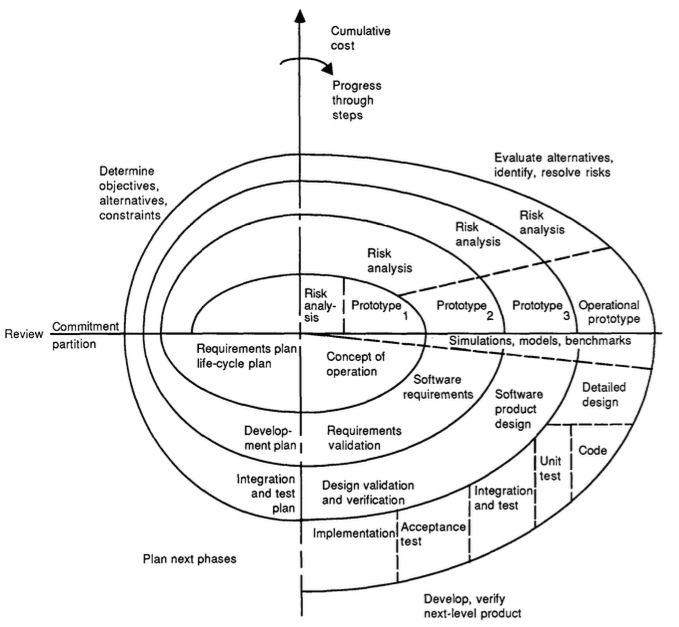
\includegraphics[width=\textwidth]{img/spiralmodell.png}
  \caption{Spiralmodell \parencite[][S. 64]{Boehm:1988aa}}
  \label{fig:spiralmodell}
\end{figure}

Bei Betrachtung der Spirale (vgl. \autoref{fig:spiralmodell}) können zwei Dimensionen für den Projektfortschritt ausgemacht werden.
Die Winkeldimension zeigt den Fortschritt einer einzelnen Iteration an, während die radiale Dimension die kumulierten Kosten bisher angibt.
\parencite[Vgl. ][S. 65]{Boehm:1988aa}

Geeignet ist das Spiralmodell für komplexe und langlaufende Projekte, bei denen sich die Anforderungen erst im Laufe der Entwicklung ergeben. 
Dabei muss jedoch beachtet werden, dass eine Gesamtplanung über die Dauer des Projekts mit steigender Anzahl an Iterationen schwieriger wird. \parencite[Vgl.][S. 58]{Schatten:2010aa}

\subsubsection{Rational Unified Process (RUP)}

RUP ist ein iterative-inkrementelles Vorgehensmodell mit den vier typischen Softwareentwicklungsphasen (vgl. \autoref{fig:rupmodell}):

\begin{itemize}
\item Konzeption
\item Entwurf und Design
\item Implementierung
\item Deployment
\end{itemize}

Das Modell setzt stark auf die Verwendung von UML und eine Toolchain zur Unterstützung \parencite[vgl.][]{Kruchten:2002:TIR:581339.581455}.

\begin{figure}
  \centering
  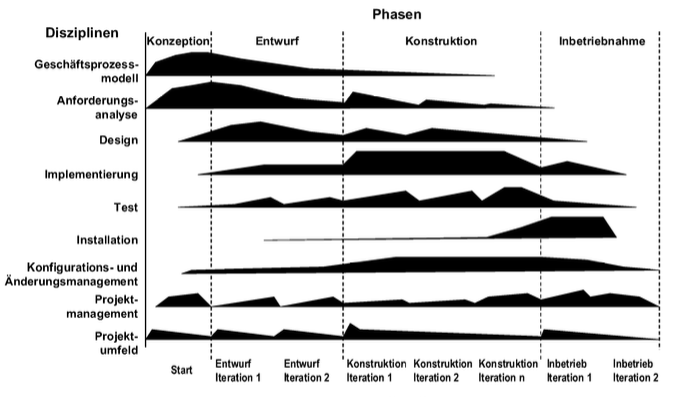
\includegraphics[width=\textwidth]{img/rupmodell.png}
  \caption{Rational Unified Process \parencite[][S. 40]{Kleuker:2011aa}}
  \label{fig:rupmodell}
\end{figure}

Jede Phase kann nochmals in mehrere Iterationen aufgeteilt werden. 
Diese werden solange wiederholt, bis ein zufriedenstellendes Ergebnis in dieser Phase erreicht wurde.
In \autoref{fig:rupmodell} können die Aufwände in der jeweiligen Phase abgelesen werden. 
Dabei ist ersichtlich, dass in jeder Phase die einzelnen Tätigkeiten unterschiedlich stark involviert sind.
Dies kann als Vorteil gegenüber dem Wasserfallmodell gesehen werden, da so z. B. Anforderungsanalyse und Test das Projekt ständig begleiten, was die Änderungsfähigkeit des Projekts begünstigt.
\parencite[][S. 60]{Schatten:2010aa} führt auf, dass insbesondere durch die Erzeugung einer Vielzahl von Dokumentation (UML etc.) die Flexibilität eingeschränkt ist.
Hierbei sollte auch bedacht werden, dass insbesondere UML als komplex und schwergewichtig bezeichnet werden kann, was dem Modell nicht zuträglich ist.

\subsubsection{V-Modell} \label{sec:vmodell}

Das V-Modell entstand durch das Bundesamt für Wehrtechnik aufgrund schlechter Erfahrungen mit anderen Vorgehensmodellen \parencite[vgl.][S. 1]{droschel2000v}.
Das V illustriert dabei die beiden Phasen \emph{Konstruktion} und \emph{Integration}.
In der Konstruktionsphase wird schrittweise das System spezifiziert und weiter verfeinert. 
Dabei liefert jede Stufe gleichzeitig die Tests für die gegenüberliegende Konstruktionsstufe.
Nach der Implementierung werden die Komponenten in der Integrationsphase stückweise integriert und gegen die zuvor spezifizierten Tests verifiziert.

\begin{figure}
  \centering
  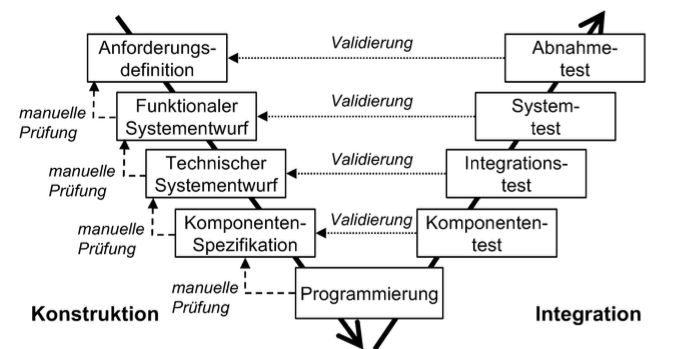
\includegraphics[width=\textwidth]{img/vmodell.png}
  \caption{V-Modell \parencite[][S. 31]{Kleuker:2011aa}}
  \label{fig:vmodell}
\end{figure}

Es lassen sich aus den einzelnen Stufen verschiedene \emph{Systemsichten} ableiten \parencite[vgl.][S. 50]{Schatten:2010aa}: 

\begin{itemize}
\item Anwendersicht (oberste Stufe)
\item Architektursicht 
\item Implementierungssicht
\end{itemize}

Das V-Modell ist ein sehr umfangreiches und komplexes Modell.
Eine ausführliche, praxisorientierte Beschreibung findet sich in \parencite[][]{brohl1993v}.
Insbesondere bei Projekten der öffentlichen Hand wird bzw. wurde das V-Modell gerne eingesetzt.
Dies liegt in der meist recht stabilen Anforderungsspezifikation dieser Projekte begründet.
\parencite[Vgl.][S. 52]{Schatten:2010aa}

\subsubsection{V-Modell XT}

Durch Erweiterung des V-Modells entstand das V-Modell XT.
Das Kürzel XT steht für \emph{Extreme Tailoring} und stellt den Fokus der Erweiterung klar: Modularität, Erweiterbarkeit und Anpassungsfähigkeit des Modells.
Ziel ist es auch, die Kommunikation zwischen Auftraggeber und Auftragsnehmer zu verbessern.
Hierfür werden Vorgehensbausteine definiert, welche flexibel kombiniert werden können \parencite[vgl.][S. 222]{Broy:2005aa}.

Das Modell ist ein Metamodell, welches den Auftragsnehmer nicht zwangsläufig dazu zwingt, das Modell genau wie angegeben durchzuführen.
Lediglich die zu liefernden Produkte in den einzelnen Phasen müssen entsprechend vorliegen.
Somit kann das Modell als eine Art Schnittstelle zwischen Auftraggeber und -nehmer angesehen werden. \parencite[Vgl.][S. 126]{Kuhrmann:2008aa}

Da, ähnlich wie beim V-Modell, sehr viel Dokumentation erzeugt wird, ist es von besonderer Wichtigkeit das Modell sehr gut anzupassen, um nicht unnötige Dokumente zu erzeugen. \parencite[Vgl.][S. 39]{Kleuker:2011aa}

Seit 2005 ist dieses Vorgehensmodell verpflichtend für alle IT-Projekte der deutschen Bundesbehörden \parencite[vgl.][]{Hohn:2008aa}.

\subsection{Agil} % 3 Seiten

In diesem Abschnitt sollen einige agile Vorgehensmodelle vorgestellt werden.
Der Grundgedanke dieser Modelle beruht auf dem agilen Manifest \parencite[][]{Beck:2001aa}:

\begin{quote}
\enquote{%
Wir erschließen bessere Wege, Software zu entwickeln,
indem wir es selbst tun und anderen dabei helfen.
Durch diese Tätigkeit haben wir diese Werte zu schätzen gelernt:

\emph{Individuen und Interaktionen} mehr als Prozesse und Werkzeuge
\emph{Funktionierende Software} mehr als umfassende Dokumentation
\emph{Zusammenarbeit mit dem Kunden} mehr als Vertragsverhandlung
\emph{Reagieren auf Veränderung} mehr als das Befolgen eines Plans

Das heißt, obwohl wir die Werte auf der rechten Seite wichtig finden,
schätzen wir die Werte auf der linken Seite höher ein.
}
\end{quote}

Ziel der agilen Vorgehensmodelle ist es, möglichst früh ein lauffähiges Inkrement zu erhalten, welches dem Kunden präsentiert werden kann. 
Dadurch soll eine enge Kollaboration mit dem Kunden erzeugt werden, so dass Änderungen möglichst schnell umgesetzt werden können. \parencite[Vgl.][S. 62]{Schatten:2010aa}

Erreicht werden sollen diese Verbesserungen offensichtlich durch die Reduzierung von unnötiger Dokumentation, enge Zusammenarbeit mit dem Kunden und einer Fokussierung auf der Generierung von Wert für den Kunden (in Form von Software).

\subsubsection{Scrum}

\emph{Scrum} ist definiert als:
\enquote{A framework within which people can address complex adaptive problems, while productively and creatively delivering products of the highest possible value}
\parencite[][S. 3]{schwaber2011scrum}.

\begin{figure}
  \centering
  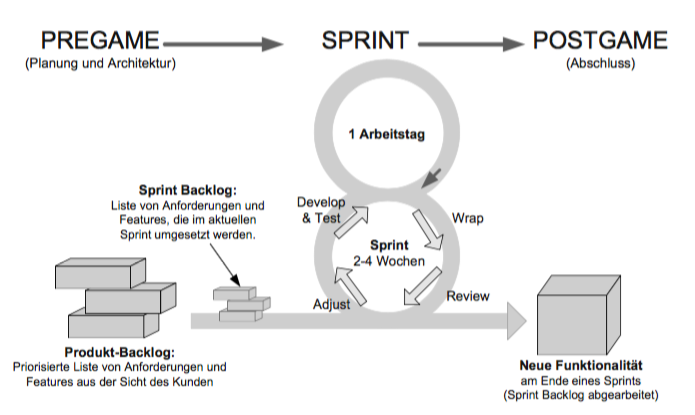
\includegraphics[width=\textwidth]{img/scrummodell.png}
  \caption{Scrum \parencite[][S. 63]{Schatten:2010aa}}
  \label{fig:scrummodell}
\end{figure}

\autoref{fig:scrummodell} visualisiert das Prinzip und den Ablauf von Scrum.
Anforderungen werden in Form von \emph{User Storys} im \emph{Product Backlog} hinterlegt.
Eine User Story beschreibt dabei ein kleines, vertikales Inkrement der Software, die dem Kunden einen Nutzen bringt.
Die selbst organisierenden Teams wählen zu Beginn eines Sprints eine Anzahl von User Storys, die sie während der Dauer des Sprints (typischerweise 2-4 Wochen) implementieren.
Am Ende eines Sprints werden die entwickelten Funktionen ausgeliefert und dem Kunden präsentiert.

Durch die kleinen Teams und kurzen Sprints wird eine hohe Flexibilität bezüglich Änderungen und der Reaktion auf Risiken erreicht.
Außerdem wird der Managementaufwand reduziert, da sich die Teams selbst organisieren.
Begleitet wird der Prozess durch einen \emph{Scrum Master}, welcher hauptsächlich organisatorische Tätigkeiten ausführt und zwischen dem Kunden und dem Team vermittelt.

So einfach das Prinzip von Scrum sein mag, so schwierig kann die Einführung in Unternehmen sein.
Es muss unterschieden werden, welche konkrete Ausprägung von Scrum bereits im Unternehmen vorherrscht und welche Ausprägung erreicht werden soll.
\parencite[][S. 8]{maximini2012scrum} beschreibt sechs Ausprägungen, die sich in der Tiefe und Nachhaltigkeit der Implementierung unterscheiden.
Das untere Spektrum wird durch \emph{Scrum PRN} (Scrum nach Bedarf) abgedeckt, welches sich durch eine spontane, lokale Umsetzung von Scrum auszeichnet.
Am anderen Ende des Spektrums steht \emph{Nachhaltiges Tiefen-Scrum}.
Hier tragen alle Mitarbeiter, die hoch motiviert sind, den Gedanken von Scrum tief in sich und treiben Veränderungen voran.

\subsubsection{Kanban}

\emph{Kanban} stammt aus dem japanischen und bedeutet sinngemäß \emph{Signalkarte} \parencite[vgl.][S. 23f.]{Epping:2011aa}.
Diese Technik stammt aus dem erfolgreichen Toyota-Produktionsprozess und stellt sicher, dass Ressourcen limitiert sind (z. B. kann ein Entwickler-Team nicht beliebig viele Features gleichzeitig umsetzen) \parencite[vgl.][S. 33f.]{Epping:2011aa}.
Meist wird ein Kanban-Board eingesetzt, welches die verschiedenen Phasen der Entwicklung visualisiert.
Dabei fließen Karten, ähnlich einer User Story, durch die Phasen des Boards.
Ziel ist es, die Durchlaufrate dieser Karten zu maximieren.
Erreicht wird dies durch eine Limitierung der Karten die sich gleichzeitig in den jeweiligen Phasen befinden können.
Dadurch werden auch Engpässe deutlich, denn wenn sich in einer Phase die Karten stauen, müssen hier die Probleme analysiert werden.

Kanban kann auch als \enquote{Wasserfallmodell im Kleinen} angesehen werden.
Ein wichtiger Unterschied ist jedoch, dass bei Kanban stets kleine Inkremente durch die Entwicklungsphasen wandern, während beim Wasserfallmodell das ganze Projekt gleichzeitig durch die Phasen wandert.

\parencite[][S. 54]{Epping:2011aa} identifiziert vier wesentliche Elemente des Kanban-Modells:

\begin{itemize}
\item Pull-Prinzip: Karten werden genommen, nicht gegeben
\item Limitierte Ressourcen
\item Transparenz: Einsicht des Projektstatus durch alle Beteiligten
\item Kontinuierliche Verbesserung
\end{itemize}

\subsubsection{Extreme Programming (XP)}

XP vereint einige der zuvor genannten agile Methoden und stellt eine Zusammenfassung bekannter Best Practices dar.
Beschrieben wurde es von Kent Beck, der explizit dazu rät, das Vorgehensmodell zuerst teilweise in einzelnen Aspekten eines Projekts einzuführen \parencite[vgl.][S. 77]{Beck:1999aa}.
Dies zeigt auch, dass XP kein formales Vorgehensmodell ist (vgl. V-Modell in \autoref{sec:vmodell}), sondern eine lose Sammlung von Methoden.
Im Fokus von XP stehen dabei Projekte die sehr ungenaue Anforderungen haben und spät im Projektverlauf noch Änderungen erfahren.
Eine grobe Beschreibung des Prozesses ist in \autoref{fig:xpmodell} ersichtlich. 

\begin{figure}
  \centering
  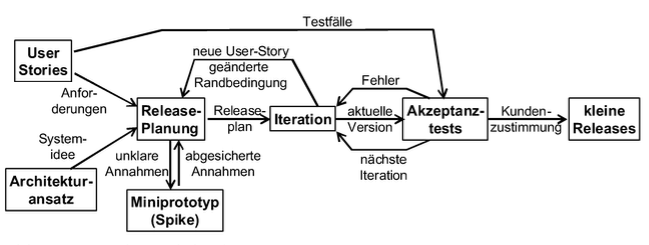
\includegraphics[width=\textwidth]{img/xpmodell.png}
  \caption{XP Prozess \parencite[][S. 46]{Schatten:2010aa}}
  \label{fig:xpmodell}
\end{figure}

Eine bekannte Praxis aus XP ist das sogenannte \emph{Pair Programming}, bei dem stets zwei Personen zusammen entwickeln.
Dies fördert die Qualität des Quellcodes und erleichtert die Erstellung von qualitativ hochwertigen Tests.
Des Weiteren kann durch diese Methode die Abhängigkeit von einzelnen Entwicklern und die Bildung von Wissenskonzentration verringert werden, da sich das Wissen auf mehrere Personen verteilt.

\section{DevOps} % 3 Seiten
Dieses Kapitel beschreibt die Situation, in der sich die Branche der klassischen Softwareentwicklung vor einigen Jahren befunden hat. Hierzu werden die damals bestehenden Probleme erörtert und eine potentielle Lösung - DevOps - näher vorgestellt.

\subsection{Ausgangslage}
Gegen Ende der 1960er Jahre befand sich die Branche der Softwareentwicklung in einer ersten ernstzunehmenden Krise. Zu dieser Zeit überschritten die Kosten für Software zum ersten Mal die Kosten von Hardware. Die zu entwickelnden Systeme hatten einen Umfang und ein Level an Komplexität erreicht, bei dem damals bewährte Vorgehensweisen an ihre Grenzen gestoßen sind. Da Kunden die Produkte erst zum Ende des Entwicklungszyklus testen und abnehmen konnten, wurden Feedback und Änderungen erst zu diesem späten Zeitpunkt bekannt. Auf Grund der hohen Komplexität der Systeme waren Änderungen zu einem so späten Zeitpunkt sehr aufwendig und kostenintensiv, oder aber überhaupt nicht mehr durchführbar. Dies führte dazu, dass sehr viele Projekte, branchenübergreifend, mit überhöhten Kosten, überschrittener Laufzeit, oder überhaupt nicht fertiggestellt werden konnten.\\
Als Reaktion darauf begann ein Umdenken in der Softwareindustrie. Auf der NATO-Konferenz 1968 in Garmisch-Partenkirchen wurde hierfür der Begriff des \glqq Software-Engineering\grqq geprägt. \parencite[Vgl.][S. 8]{Naur:1968} Es wurden Vorgehensweisen und Methoden entwickelt, die sich an bereits etablierte Ingenieursdisziplinen orientiert haben. Diese basierten auf ausführlicher Planung und Dokumentation. Eine Folge dessen war die Bildung unterschiedlicher Abteilungen und Spezialisierungen von Berufen innerhalb von Firmen. So entstand eine Trennung von Anforderungsmanagement und Umsetzung der einzelnen Projekte. Durch diese Standardisierung konnte zwar die Planbarkeit von Projekten deutlich gesteigert werden, jedoch wurden Projekte sehr anfällig für ungenau, oder fehlerhaft erfasste Anforderungen. Auch die Umsetzung von Änderungswünschen der Kunden wurden zunehmend schwieriger und kostenintensiver, je später sie im Projektverlauf auftraten. Diese klassischen Entwicklungsprozesse beinhalten auch ein Änderungsmanagement, welches aber mit großem Aufwand bei Anforderungserfassung, Dokumentation und Kommunikation verbunden ist.\\
Als Antwort auf diese Probleme entstand agile Softwareentwicklung. Hierbei wird Software iterativ und inkrementell entwickelt. Es werden regelmäßig lauffähige Prototypen an den Kunden ausgeliefert und dessen Feedback eingeholt und in die Entwicklung integriert. Dadurch ist es möglich, flexibel auf Änderungen seitens des Kunden einzugehen. \glqq Auslöser der agilen Methoden war das Gefühl, durch Bürokratie, Prozesse und Dokumentationsvorgaben gelähmt und gehemmt zu werden. Gerade schnelle, risikoreiche und damit auch chancenreiche Projekte schienen darunter zunehmend zu leiden.\grqq \parencite[Vgl.][S. 183]{Schneider:2007}
Im Zuge der Ausbreitung der agilen Vorgehensweisen wurde die Entwicklung von Software flexibler und die Kommunikation mit Kunden und innerhalb der Entwicklungsteams deutlich verbessert. Allerdings beschränken sich diese Prozesse und Vorgehensweisen lediglich auf die Anforderungserfassung und Entwicklung, jedoch nicht auf die Qualitätssicherung und den Betrieb der Systeme. Diese stellen in vielen Unternehmen immer noch getrennte Abteilungen dar mit entsprechenden Schwierigkeiten in der Organisation. So besteht innerhalb vieler Abteilungen ein starkes Zusammengehörigkeitsgefühl, jedoch eine meist ebenso große Abgrenzung zu anderen Abteilungen hin. Dies führt oft dazu, dass Probleme einfach weitergereicht werden und nur der eigene Vorteil, nicht jedoch der Vorteil der Gemeinschaft, im Vordergrund steht. Zudem konzentriert sich bei der Bildung sogenannter Silos Wissen in sehr stark beschränkten Grenzen. Da die Informatik, im Vergleich zu anderen Ingenieursdisziplinen, immer noch eine sehr junge Disziplin ist, befindet sich diese in stetigem Wandel und kontinuierlicher Optimierung. Besonderer Fokus liegt auf der Organisation und auf Vorgehensmodellen zur Softwareentwicklung. Aus den Erfahrungen, die mit agilen Prozessen gewonnen wurden und diesem Streben nach Weiterentwicklung entstand DevOps. \parencite[Vgl.][]{Debois:2008}\\

\subsection{Geschichte und Entwicklung des Begriffs}
DevOps ist eine Weiterentwicklung der agilen Idee beziehungsweise der agilen Vorgehensweise und eine Ausweitung dieser auf weitere Bereiche wie die Qualitätssicherung und den Betrieb von Softwaresystemen. Der Begriff setzt sich aus den Worten \glqq Development\grqq und \glqq Operations\grqq zusammen.

\begin{figure}[ht]
  \centering
  \includegraphics[width=0.5\textwidth]{img/devops_graphic.png}
  \caption{Zusammensetzung (Entwicklung, Qualitätssicherung und Betrieb)}
  \label{fig:devops_composition}
\end{figure}

Die Vorgehensweise, die DevOps beschreibt, wurde erstmals auf der Agile 2008 Konferenz von Patrick Debois im Beitrag \glqq Agile Infrastructure \& Operations\grqq erwähnt. \parencite[Vgl.][]{Debois:2008} Der Begriff \glqq DevOps\grqq verbreitete sich in den darauf folgenden Jahren durch eine Serie von Konferenzen, genannt \glqq devopsdays\grqq.
DevOps selbst entstand aus unterschiedlichen Bewegungen wie \glqq Infrastructure as Code\grqq, \glqq Agile Infrastructure\grqq, \glqq Agile System Administration\grqq, \glqq Lean Startup\grqq und \glqq Continuous Integration and Release\glqq. \parencite[Vgl.][S. 4]{Kim:2015}
Die Verbreitung von DevOps war in den ersten Jahren sehr gering und fast ausschließlich auf die Bereiche des Cloud Computing und mobiler Entwicklung beschränkt \parencite[Vgl.][]{Gartner:2015}, da die Vorteile von DevOps in diesen Bereichen gegenüber den bisherigen Vorgehensweisen am größten sind. Besonders in den Jahren 2014 und 2015 wuchs das Interesse an DevOps immer mehr an. \parencite[Vgl.][S. 7]{DevOpsSODR:2015} Mittlerweile findet DevOps Einsatz in 25 Prozent aller IT weltweit und für das Jahr 2016 ist ein Wachstum auf bis zu 25 Prozent vorhergesagt. \parencite[Vgl.][]{Gartner:2015} Das steigende Wachstum der Verbreitung von Devops ist auch der Tatsache geschuldet, dass die Tools, die im Umfeld von DevOps entstanden sind auch in anderen Vorgehensmodellen und Prozessen, besonders in agilen Prozessen, zum Einsatz kommen können und auch vielfach eingesetzt werden.

\subsection{Ziele}
DevOps ist, wie bereits zuvor erwähnt, eine Weiterentwicklung der agilen Softwareentwicklung. Hierbei wird der agile Gedanke auf weitere Bereiche wie Qualitätssicherung und Betrieb übertragen. DevOps definiert dabei als wichtigste Ziele:

\begin{itemize}
\item Steigerung der Kommunikation und Kollaboration, insbesondere zwischen Entwicklung und Betrieb
\item Steigerung der Qualität des Produkts mit erhöhter Stabilität, Sicherheit und Zuverlässigkeit
\item Automatisierung des Entwicklungsprozesses und der Auslieferung für eine kurze Time To Market
\end{itemize}
\parencite[Vgl.][S. 4]{Kim:2015}

Betrachtet wird die Umsetzung dieser Ziele von DevOps auf den folgenden drei Ebenen: 

\begin{itemize}
\item Organisatorisch
\item Technisch
\item Kulturell
\end{itemize}

Auf organisatorischer Ebene steht bei DevOps die Vereinigung unterschiedlicher Bereiche im Vordergrund. Hierzu muss ein gemeinsames Management der Abteilungen Entwicklung, Qualitätssicherung und Betrieb geschaffen werden und die Teams müssen entsprechend zusammengesetzt werden. Dies führt dazu, dass es keine reinen Experten mehr für bestimmte Bereiche gibt, sondern, dass jedes Teammitglied Wissen auf allen drei Gebieten besitzen muss. Dies schließt jedoch nicht aus, dass Teammitglieder immer noch bestimmte Kompetenzschwerpunkte besitzen. Durch die Zusammenfassung der Organisation wird versucht, die Kommunikation und Kollaboration innerhalb des Teams zu verbessern und somit ein qualitativ hochwertigeres Produkt zu schaffen, schneller auf Fehler reagieren zu können und eine schnellere Time To Market zu erreichen.\\
Auf technischer Ebene wird besonders die Steigerung der Qualität des Produkts und die Automatisierung des Entwicklungsprozesses und der Auslieferung unterstützt. Das Kernstück bildet hierbei eine Continuous Delivery Pipeline, in die automatisierte Tests eingebunden werden können. In Kombination mit automatisiertem Deployment können somit sowohl die Time To Market, als auch die Time To Recover sehr stark verkürzt werden. Zudem wird die Verwaltung der Produktion vereinfacht und optimiert, da alle erstellten Artefakte in einer zentralen Quellcodeverwaltung gespeichert werden. Mit Hilfe dieser technischen Mittel werden alle Vorgänge und Änderungen protokolliert und beliebig reproduzierbar.\\
Eine Ebene, die im Zusammenhang mit DevOps oftmals vernachlässigt wird, der aber essentiell wichtig ist, ist die kulturelle Ebene. Diese bildet das ideologische Herzstück von DevOps. Organisatorische Änderungen und der Einsatz technischer Hilfsmittel bringt zwar ebenso gewisse Vorteile, in vollem Umfang nutzbar sind diese jedoch nur mit entsprechender Verankerung in der Organisationskultur. Hierbei steht besonders die Definition eines gemeinsamen Ziels im Fokus. Die angestrebte Form der Organisation ist eine generative und leistungsorientierte Organisation, die ein motivierendes, innovatives und fehlerverzeihendes Umfeld bietet, die Kollaboration fördert und das Produkt zum gemeinsamen Ziel der Organisation macht. Alle Teammitglieder tragen gemeinsam die Verantwortung für die Entwicklung, die Qualität und den Betrieb des Produkts.

\section{Klassische und sicherheitskritische Bereiche im Vergleich} \label{sec:bereiche} % 4 Seiten

In diesem Abschnitt sollen klassische und sicherheitskritische Bereiche bezüglich relevanter Faktoren wie dem Sicherheitsanspruch an die Software, den bestehenden Normen, vorherrschenden Entwicklungspraktiken und der Time To Market verglichen werden.

\subsection{Sicherheitsanspruch} % 1 Seite

Die Bewertung von Bugs in Software hängt von dem betrachteten Bereich ab.
Fehler in Software für klassische Bereiche haben meist nur hohe monetäre Kosten.
So haben beispielsweise die Viren MyDoom, SoBig.F, Slammer, etc., die Software Bugs ausgenutzt haben, weltweit einen finanziellen Schaden von mehreren Milliarden Euro verursacht. \parencite[Vgl.][]{ComputerEconomics2004aa}

Dahingegen sind die Folgen von Fehlern in sicherheitskritischen Bereichen weitaus schwerwiegender, denn beispielsweise Fehler in Satelliten können nicht einfach ausgebessert werden, diese müssen sofort fehlerfrei arbeiten.
\parencite[][S. 87 - 89]{Zhivich:2009aa} nennt mehrere große Ereignisse in sicherheitskritischen Bereichen mit teilweise fatalen Folgen:

Ein Berechnungsfehler durch Missachtung der beschränkten Präzision von Gleitkommaoperationen führte bei einem Patriot-Raketen-Abwehrsystem der US-Armee in Saudi-Arabien zum Tod von 28 Soldaten.
Eine Scud-Rakete\footnote{Russische Boden-Boden-Kurzstreckenrakete} konnte aufgrund des Fehlers nicht abgefangen werden, da die Flugbahn der Rakete falsch bestimmt wurde.
Ursache war einerseits der Berechnungsfehler, andererseits eine fehlerhafte Verwendung.
Das System war für eine Betriebsdauer von 14 Stunden spezifiziert, wurde in Saudi-Arabien jedoch rund 100 Stunden ununterbrochen benutzt.
Dadurch summierte sich der Berechnungsfehler auf und führte zu der fehlerhaften Flugbahnberechnung.

Ein weiterer Vorfall ereignete sich im medizinischen Bereich.
Durch eine Race-Condition\footnote{Ablauf von nebenläufigen Operationen, deren Ergebnis von der Reihenfolge abhängt.} in einem Bestrahlungsgerät wurden Krebspatienten mit der hundertfachen Dosis bestrahlt.
Die Race-Condition konnte ausgelöst werden, wenn das Bedienpersonal am Gerät zu schnell verschiedene Tasten betätigte, was einen inkonsistenten Zustand zwischen Display und tatsächlichem Status des Geräts zur Folge hatte.

Auch Bedrohungen für die Infrastruktur können auftreten, wie ein Bruch einer Gas-Pipeline in den USA beweist.
Zwar war der Hauptgrund ein physischer Defekt, jedoch hätte das Kontrollsystem dies anzeigen müssen.
Aufgrund eines nicht näher genannten Fehlers war dies nicht der Fall und das Personal konnte den Fehler nicht rechtzeitig entdecken.
Andernfalls hätte die Pipeline vorher abgeschaltet und der Tod von drei Menschen verhindert werden können.

Diese Vorfälle zeigen deutlich, wie unterschiedlich die Anforderungen an die Sicherheit von Software in klassischen bzw. sicherheitskritischen Bereichen sind.

\subsection{Normen} % 2 Seiten

In den klassischen Bereichen existiert meist keine bindende Norm für die Unternehmen.
Jedoch bietet die Norm DIN ISO/IEC 12119 einen Katalog an Anforderungen, der eine gewisse Qualität der Software garantiert.
So wird z. B. auf Endlosschleifen, Abstürze, Bedienbarkeit, Benutzerdokumentation und korrekte Versionierung geprüft. 
Eine weitere Norm die allgemeine Qualitätsanforderungen stellt ist die ISO 9001.
Diese ist jedoch weniger auf das Endprodukt als auf die Entwicklung und Organisation ausgerichtet.
\parencite[Vgl.][S. 66 - 67]{Hohler:1998aa}


Für sicherheitskritische Bereiche existieren einige spezielle Normen wie beispielsweise die ECSS-E-40 Norm der European Corporation on Space Standardization (ECSS).
Vorläufer bzw. Basis der Norm ist ISO 12207.
Hauptfokus der Norm ist die Definition von Prozessen und deren Beschreibung. 
Die Norm beschreibt die Anforderungen und die erwarteten Eingabe und Ergebnisse der Prozesse.

Dabei ist stets zu beachten, dass die Norm versucht möglichst flexibel zu sein und so ermöglicht, eigene Vorgehensweisen auf diese Norm zu übertragen bzw. anzupassen (\emph{tayloring}).
Grundlegend ist das Lieferant-Kunden-Konzept, welches mehrstufig die involvierten Unternehmen im Entwicklungsprozess als Lieferant bzw. Kunde ansieht und die Austauschpunkte in Form von Reviews gestaltet.
Die Prozesse umfassen:

\begin{description}
\item[System Engineering] Umfasst Systemanforderungsanalyse, -integration und -validierung. 
Wird durch den Kunden ausgeführt.
\item[Software Requirements Engineering] Erstellung einer Softwareanforderungsanalyse und eines Architekturdesign durch den Lieferanten.
\item[Software Design Engineering] Implementierung, Testen, Integrieren und Validieren der Softwarekomponenten durch den Lieferanten.
\item[Software Validation and Acceptance] Validierung gegen die Anforderungen, Deployment und Akzeptanztest.
\item[Software Operations Engineering] Vorbereiten des Betriebs der Software, der operationellen Tests und des Benutzersupport.
\item[Software Maintenance] Problemanalyse, Bugfixing, Migration und Abschaltung von Software.
\end{description}

\begin{figure}
  \centering
  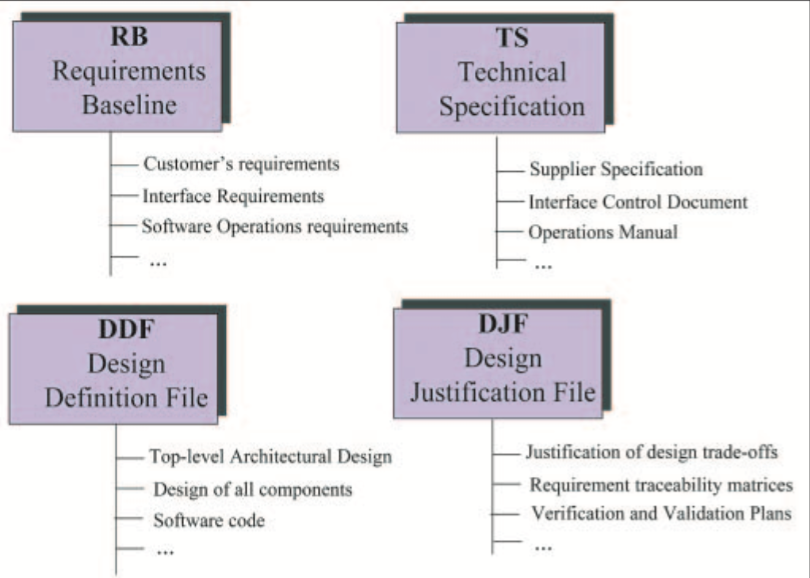
\includegraphics[width=0.8\textwidth]{img/ecss-dokumentation.png}
  \caption{Dokumentationskategorien von ECSS-E-40 \parencite[][S. 136]{jones2002introducing}}
  \label{fig:ecss-dok}
\end{figure}

Kennzeichnend ist die Maßgabe, dass sehr viel und ausführlich dokumentiert werden muss.
Eine Vielzahl von Kategorien (vgl. \autoref{fig:ecss-dok}) zeigt die strengen Dokumentationsanforderungen.
Der Standard legt Wert darauf, dass insbesondere die Anforderungen von Raumfahrtsoftware, wie begrenzte Ressourcen und gestiegene Komplexität möglichst gut abgedeckt werden.
\parencite[Vgl.][]{jones2002introducing}

Die Norm RTCA/DO-178B ist speziell für die Software in Flugzeugen definiert.
Diese ebenfalls prozessorientierte Norm betrachtet auch externe Software (z. B. Entwicklungsumgebungen).
Im Organisationsprozess wird die Anforderungsklasse der Software aus den Anforderungen an das Gesamtsystem abgeleitet, der Softwarelebenszyklus und die Dokumentation spezifiziert.
\parencite[Vgl.][S. 71]{Hohler:1998aa}

Im Softwarelebenszyklus werden dabei die einzelnen Phasen während der Entwicklung und des Betriebs der Software beschrieben.
Der Softwareentwicklungsprozess umfasst die Anforderungsanalyse, Implementierung, Integration und Validierung, wobei die Validierung Reviews, Analysen und Tests beinhaltet.
Während der Reviews und Analysen wird geprüft, ob alle organisatorischen (Dokumentation etc.) und fachlichen (Algorithmen etc.) Anforderungen eingehalten wurden.
\parencite[Vgl.][S. 71]{Hohler:1998aa}

Die Testphase erfordert das Durchführen von White-, Black-Box (mit Äquivalenzklassenbildung) und Integrationstests.
Zusätzlich ist die Implementierung eines Konfigurationsmanagementprozesses erforderlich, um die Kombinationen von Software und Hardware zu verwalten.
\parencite[Vgl.][S. 71]{Hohler:1998aa}

Häufig in der Raumfahrt verwendet wird der Standard IEC 61508 Teil 7.
Dieser beschreibt welche Methoden für die Raumfahrt und andere sicherheitskritische Bereiche geeignet sind.
Der Fokus liegt wie bei den meisten anderen Normen auf eingebetteten Systemen.
Abgeleitet von diesem Standard wurde RTCA/DO-178B.
Ziel der Norm ist es, die Risiken während des Betriebs der Software zu minimieren.
\parencite[Vgl.][S. 40]{Carpenter:2014aa}

\subsection{Entwicklungspraktiken} % 1-2 Seiten

Sicherheitskritische Bereiche setzen bei der Entwicklung üblicherweise auf ein sehr formales, geplantes Vorgehen.
Frameworks helfen alle erforderlichen Prozesse und Zwischenprodukte zu durchlaufen bzw. zu generieren.
Ein weitere Vorteil von Frameworks, die dies unterstützen, ist, dass komplexe Software von mehreren Lieferanten in den Entwicklungsprozess eingebunden werden kann.
Meist nutzen diese eigene Entwicklungsprozesse und Vorgehensmodelle.
Durch ein Framework lassen sich diese über wohldefinierte Schnittstellen einbinden.
Dies umfasst eine umfangreiche und exakte Dokumentation aller Softwareprodukte.
\parencite[Vgl.][S. 39]{Carpenter:2014aa}

Zusätzlich wird durch Redundanz versucht die Auswirkungen von Fehlern zu minimieren.
So könnte ein zweites Steuerungssystem in einem Flugzeug Leben retten, wenn das erste aufgrund eines Hardware- oder Softwaredefekts ausfällt.
Auch die Wiederverwendung von Komponenten spielt in diesen hochspezialisierten Bereichen eine geringere Bedeutung, während in klassischen Bereichen oft Wert auf Wiederverwendung gelegt wird, um neue Produkte schneller und günstiger herstellen zu können.
\parencite[Vgl.][S. 39]{Carpenter:2014aa}

Auch bezüglich der Vorgehensmodelle sind sicherheitskritische Bereiche wesentlich konservativer eingestellt.
Um den Anspruch einer umfangreichen Dokumentation zu erfüllen wird meist auf klassische Vorgehensmodelle gesetzt.
\parencite[Vgl.][S. 39]{Carpenter:2014aa}

Die Best Practices für Raumfahrtentwicklung zeigen den starken Formalismus in der Entwicklung auf \parencite[vgl.][S. 269ff]{Hersman:2010aa}.
Geprägt durch eine Vielzahl an Normen, Zertifizierungen und Prozessen wird auf die besonderen Anforderungen dieses Bereichs Rücksicht genommen.

Dem gegenüber steht ein weniger formales, flexibleres Vorgehen in den klassischen Bereichen. 
Als Grund lassen sich kürzere Entwicklungszeiten, hoher Wettbewerbsdruck und niedrigere Risiken identifizieren (vgl. \autoref{sec:bereiche}).


\subsection{Time To Market} % 1/2 Seite

In der Raumfahrtindustrie sind die Entwicklungszeiten wesentlich länger im Vergleich zu klassischen Bereichen.
Die Projektplanung bzw. die Einhaltung des Plans habe in diesen Bereichen das größte Gewicht. 
Hier gilt es, möglichst schnell unter Zeitdruck vor den Mitbewerbern ein lauffähiges Produkt auszuliefern.
Dabei belaufen sich die Entwicklungszeiten meist auf wenige Monate bis Jahre (selten).
Dahingegen sind in der Raumfahrtindustrie lange Laufzeiten von mehreren Jahren der Regelfall.
Des Weiteren ist der Schwerpunkt mehr auf Qualität und Funktionsumfang gesetzt, was sich auch in einem erhöhten Bürokratieaufwand niederschlägt.
\parencite[Vgl.][S. 97]{Dorfman:1999aa}


